% !TEX root = ../foresight.tex

\section{Results}

\subsection{Localization Accuracy}

We tested our localization framework by emulating the car's ultra-wideband
sensor configuration inside a motion capture system. We placed motion capture
markers on the quadrotor and on each ultra-wideband sensor. This allowed us to
obtain the absolute position of the quadrotor and UWBs in the same coordinate
frame. We then flew the quadrotor inside the motion capture system and recorded
its predicted position determined by our localization and absolute position
using the motion capture markers. The average error in our localization was
13.7 cm, or 35.9\% the length of the quadrotor. Fig.~\ref{fig:localization}
shows how our localization compares to the ground truth. The green and red
lines respectively show the ground truth and predicted positions of the
quadrotor.

\begin{figure}

    \centering

    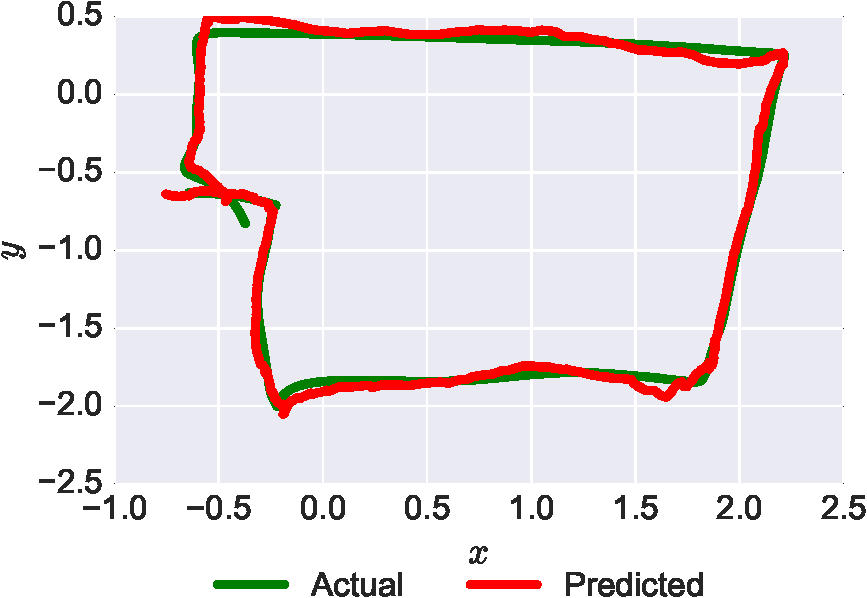
\includegraphics[width=0.7\linewidth]{localization}

    \caption{Plot showing the how our localization method compares to the
    ground truth. Ground truth was supplied by a motion capture system.}

    \label{fig:localization}

\end{figure}

\subsection{Experimental Setup}

For our experiments, we used a Toyota Prius with a SICK LMS1xx mounted on the
front of the car and six Decawave TREK1000 ultra-wideband radios mounted on the
roof and front bumper of the car. A platform for the quadrotor to take off and
land is attached to the front bumper of the Prius. We used a Parrot Bebop 2
quadrotor with a Decawave TREK1000 mounted on the battery.  Fig.~\ref{fig:car}
and Fig.~\ref{fig:bebop-actual} show the Toyota Prius and modified Bebop 2
quadrotor used the experiments.

\begin{figure}[h!]

    \centering

    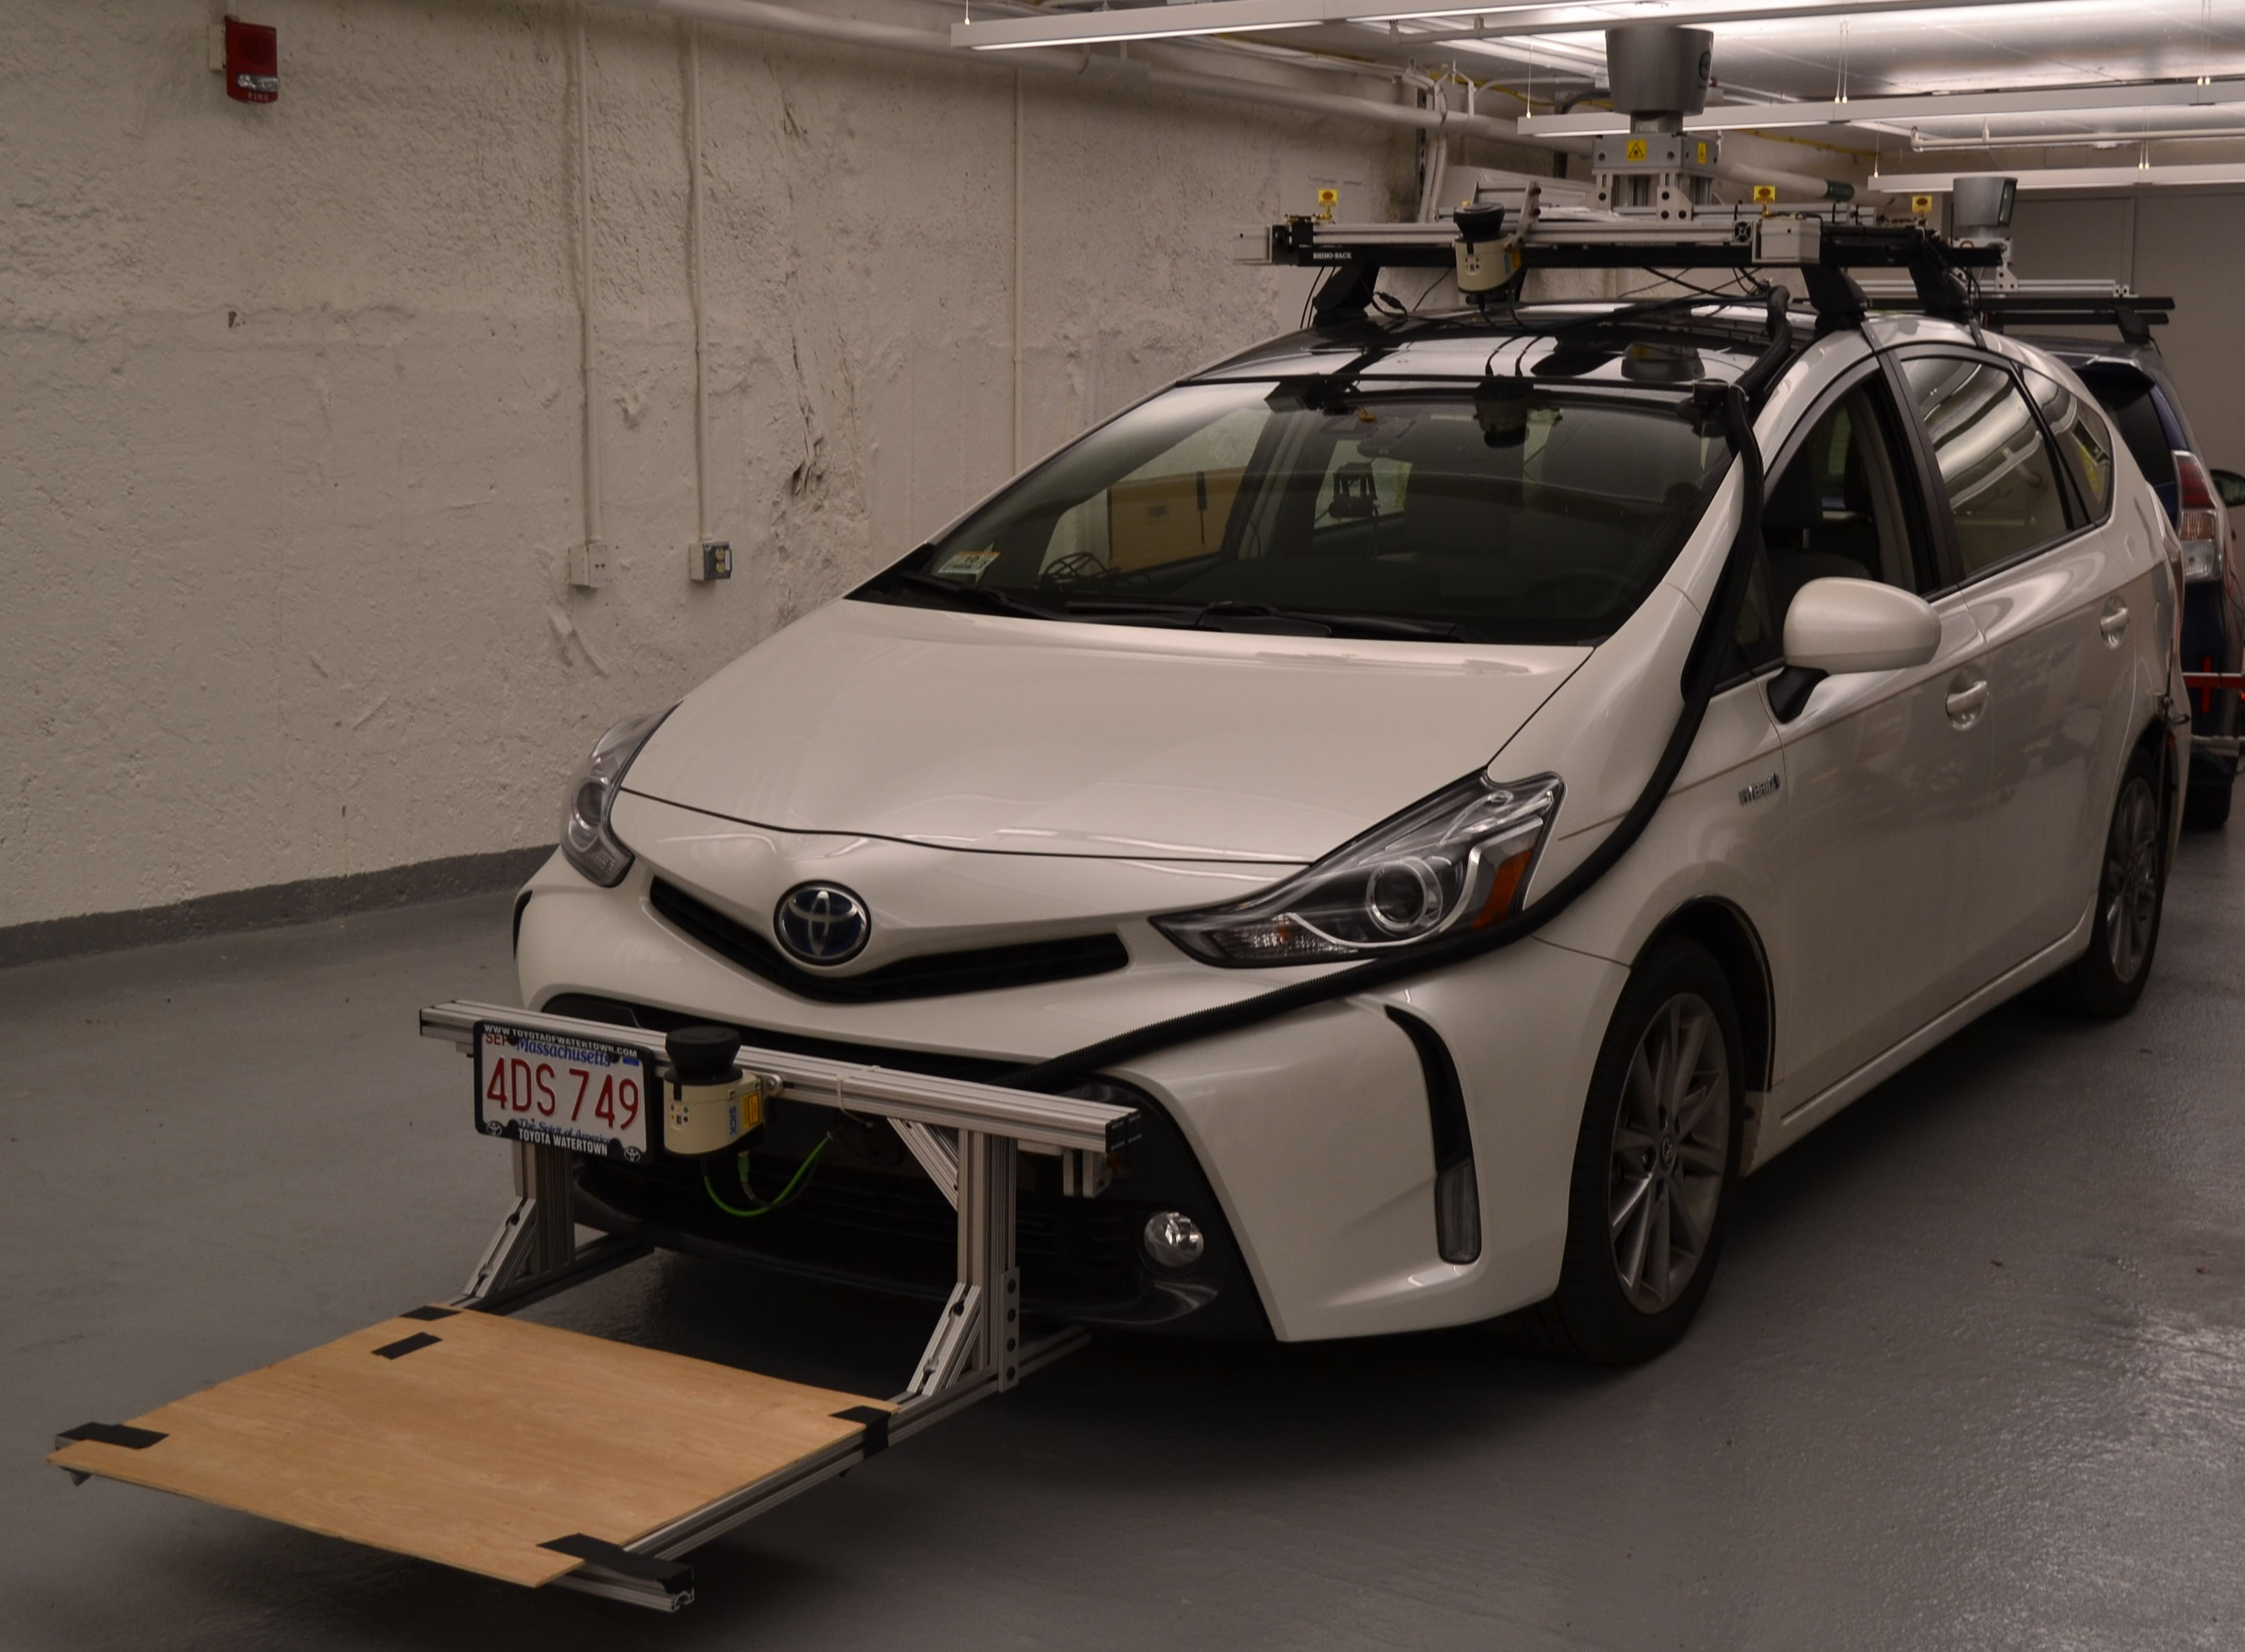
\includegraphics[width=0.9\linewidth]{car}
    % 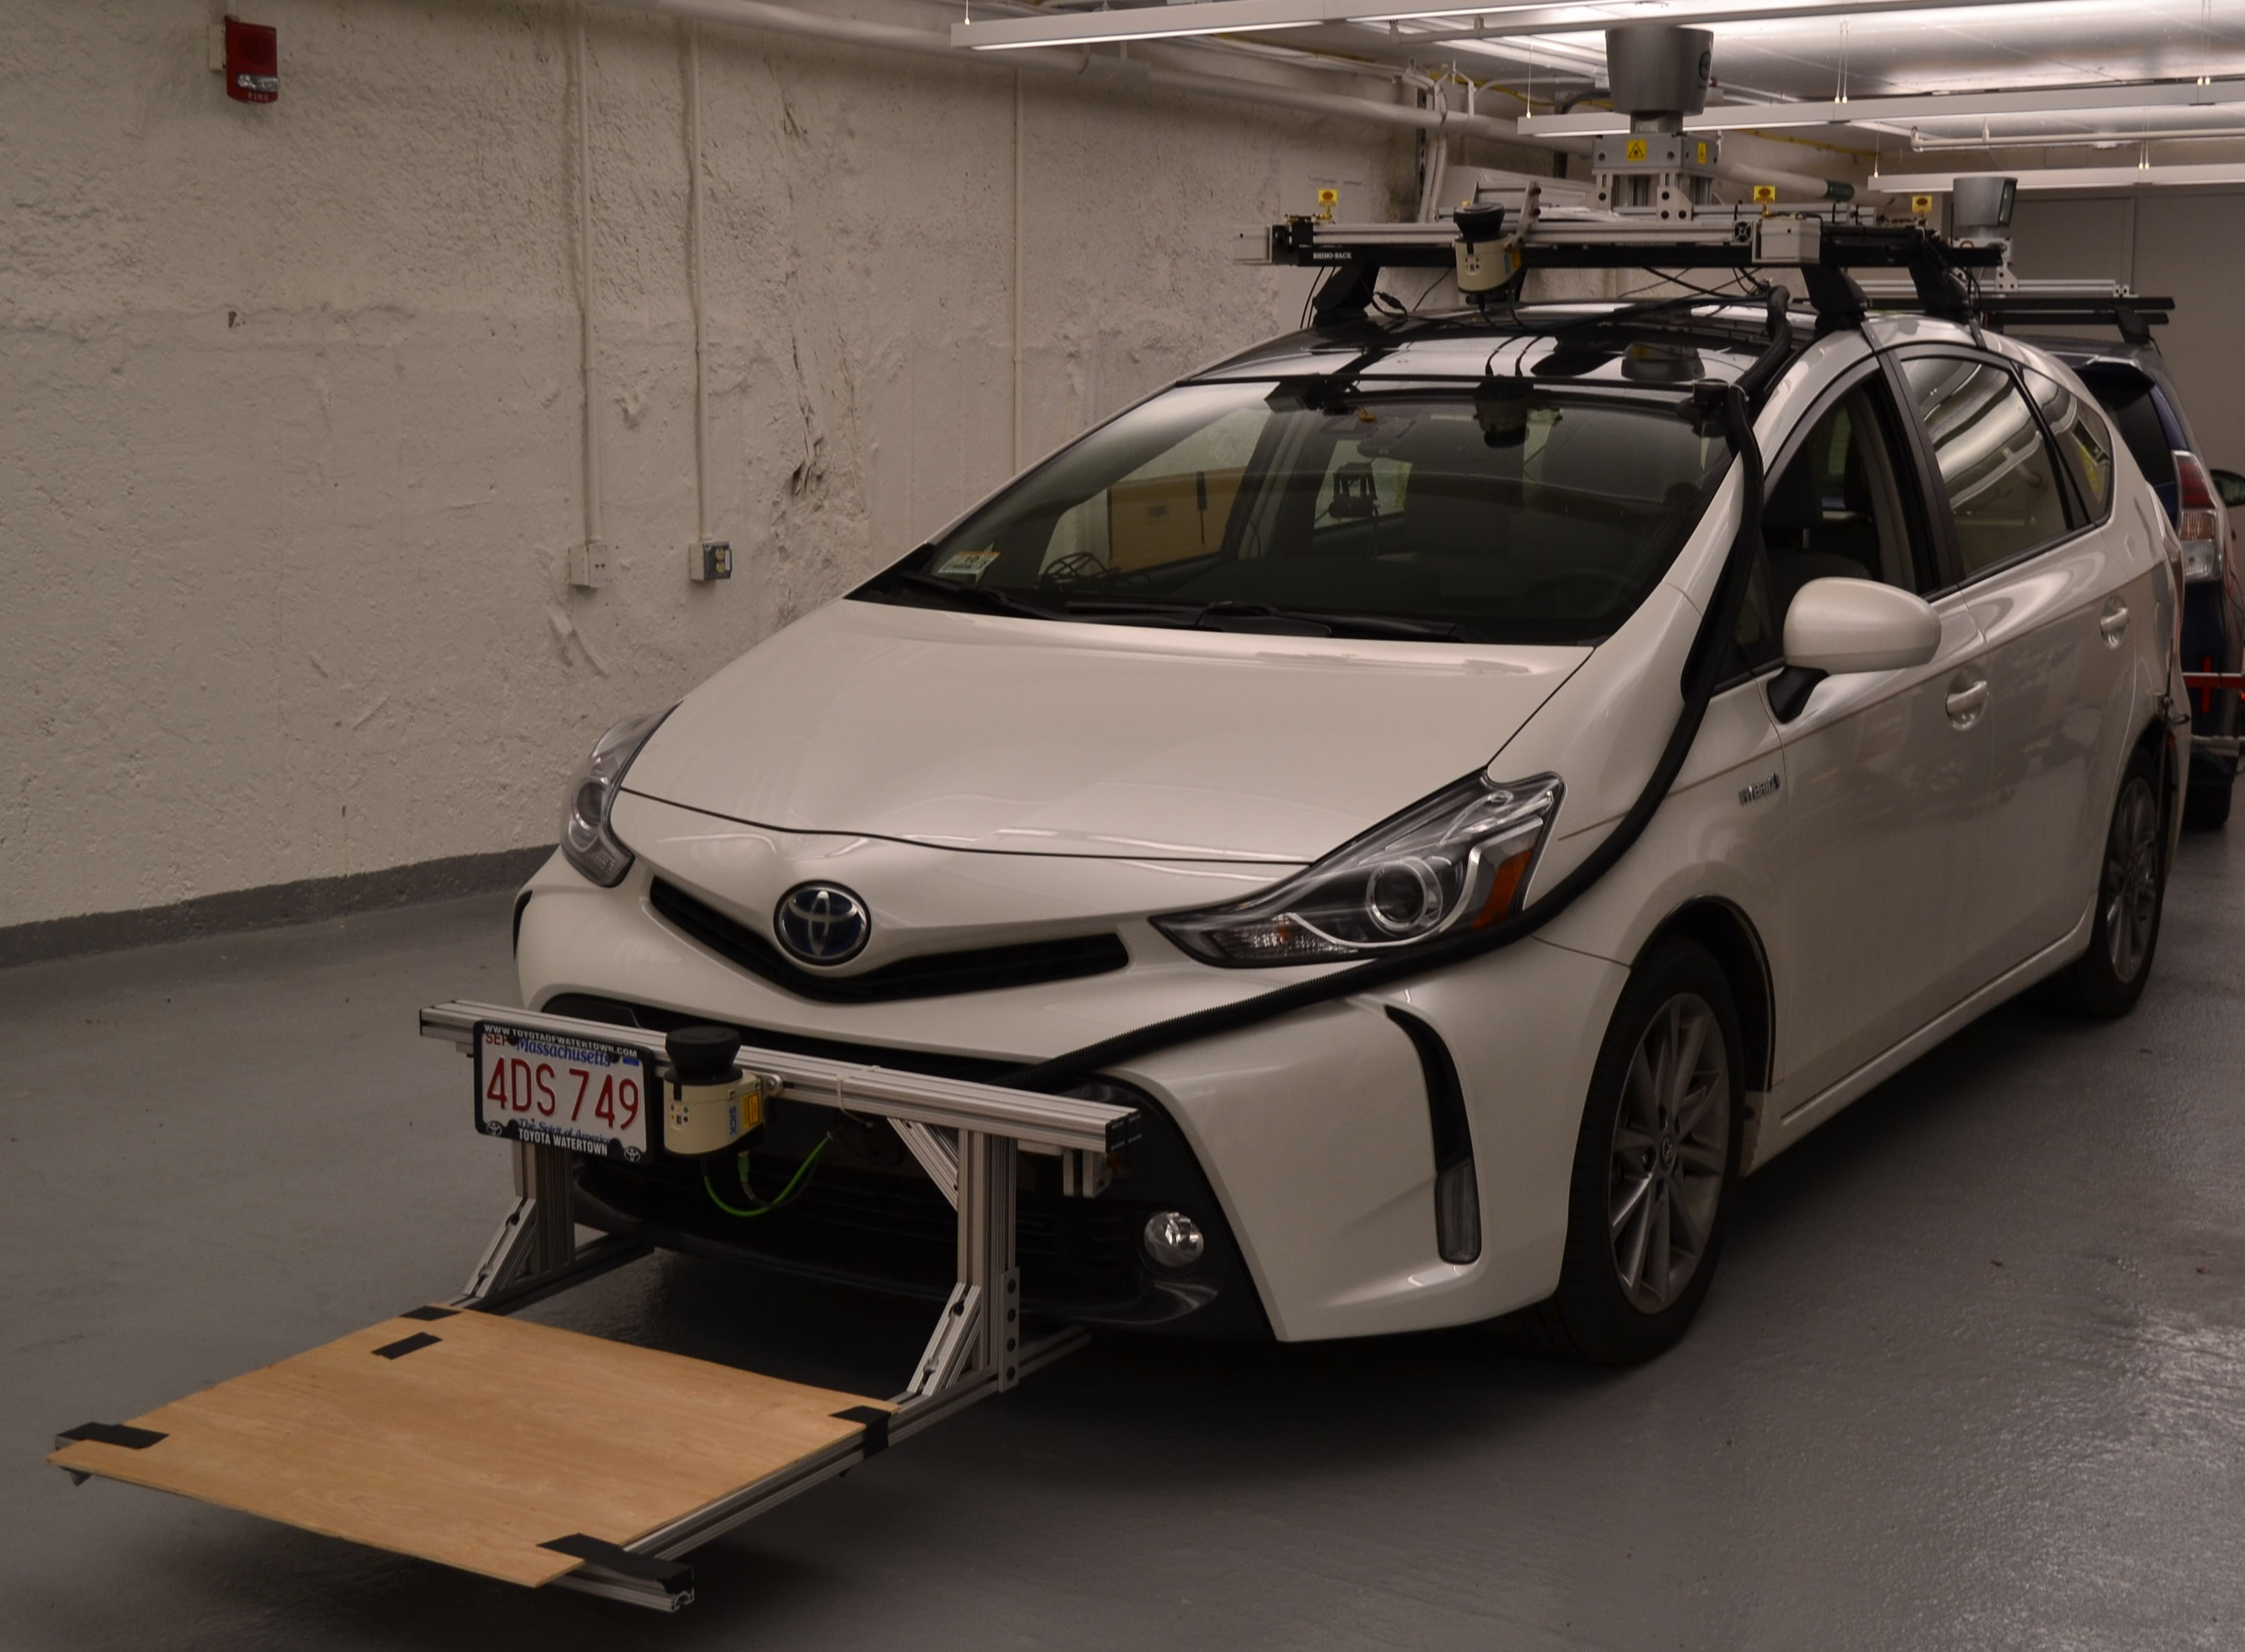
\includegraphics[height=3.8cm]{car}
    % 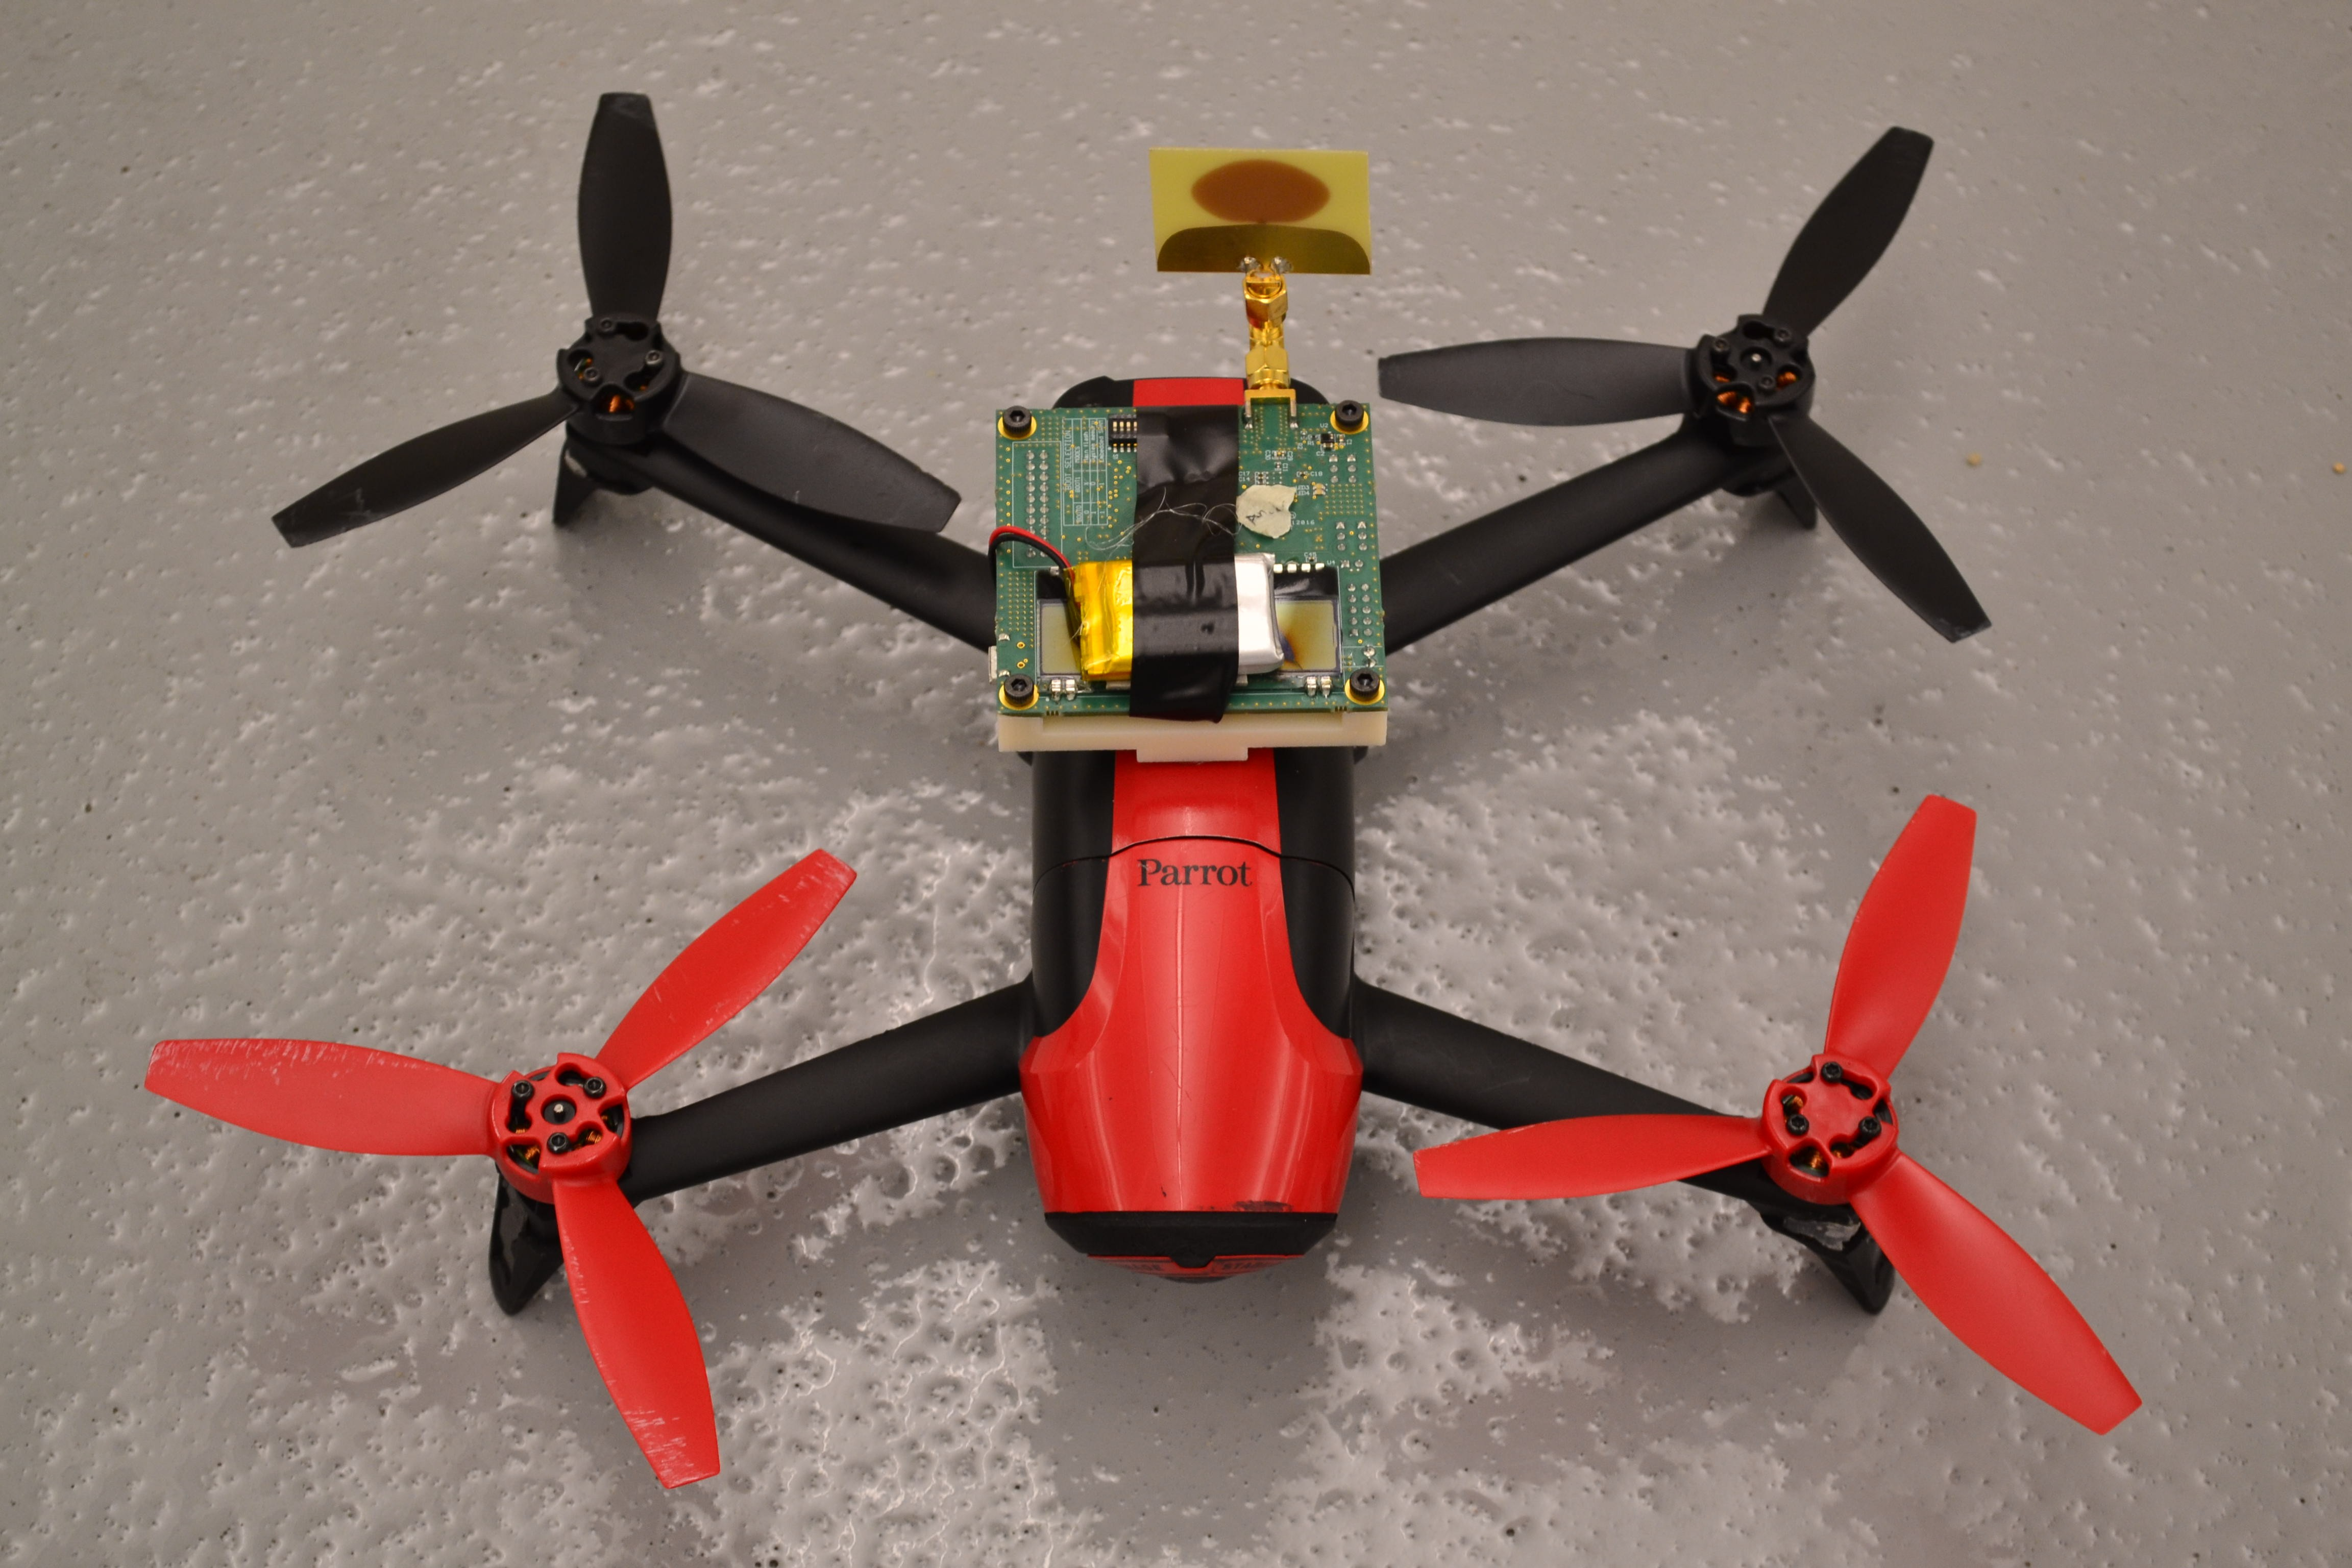
\includegraphics[height=3.8cm]{bebop-actual}

    \caption{}

    \label{fig:car}

\end{figure}

\begin{figure}[h!]

    \centering

    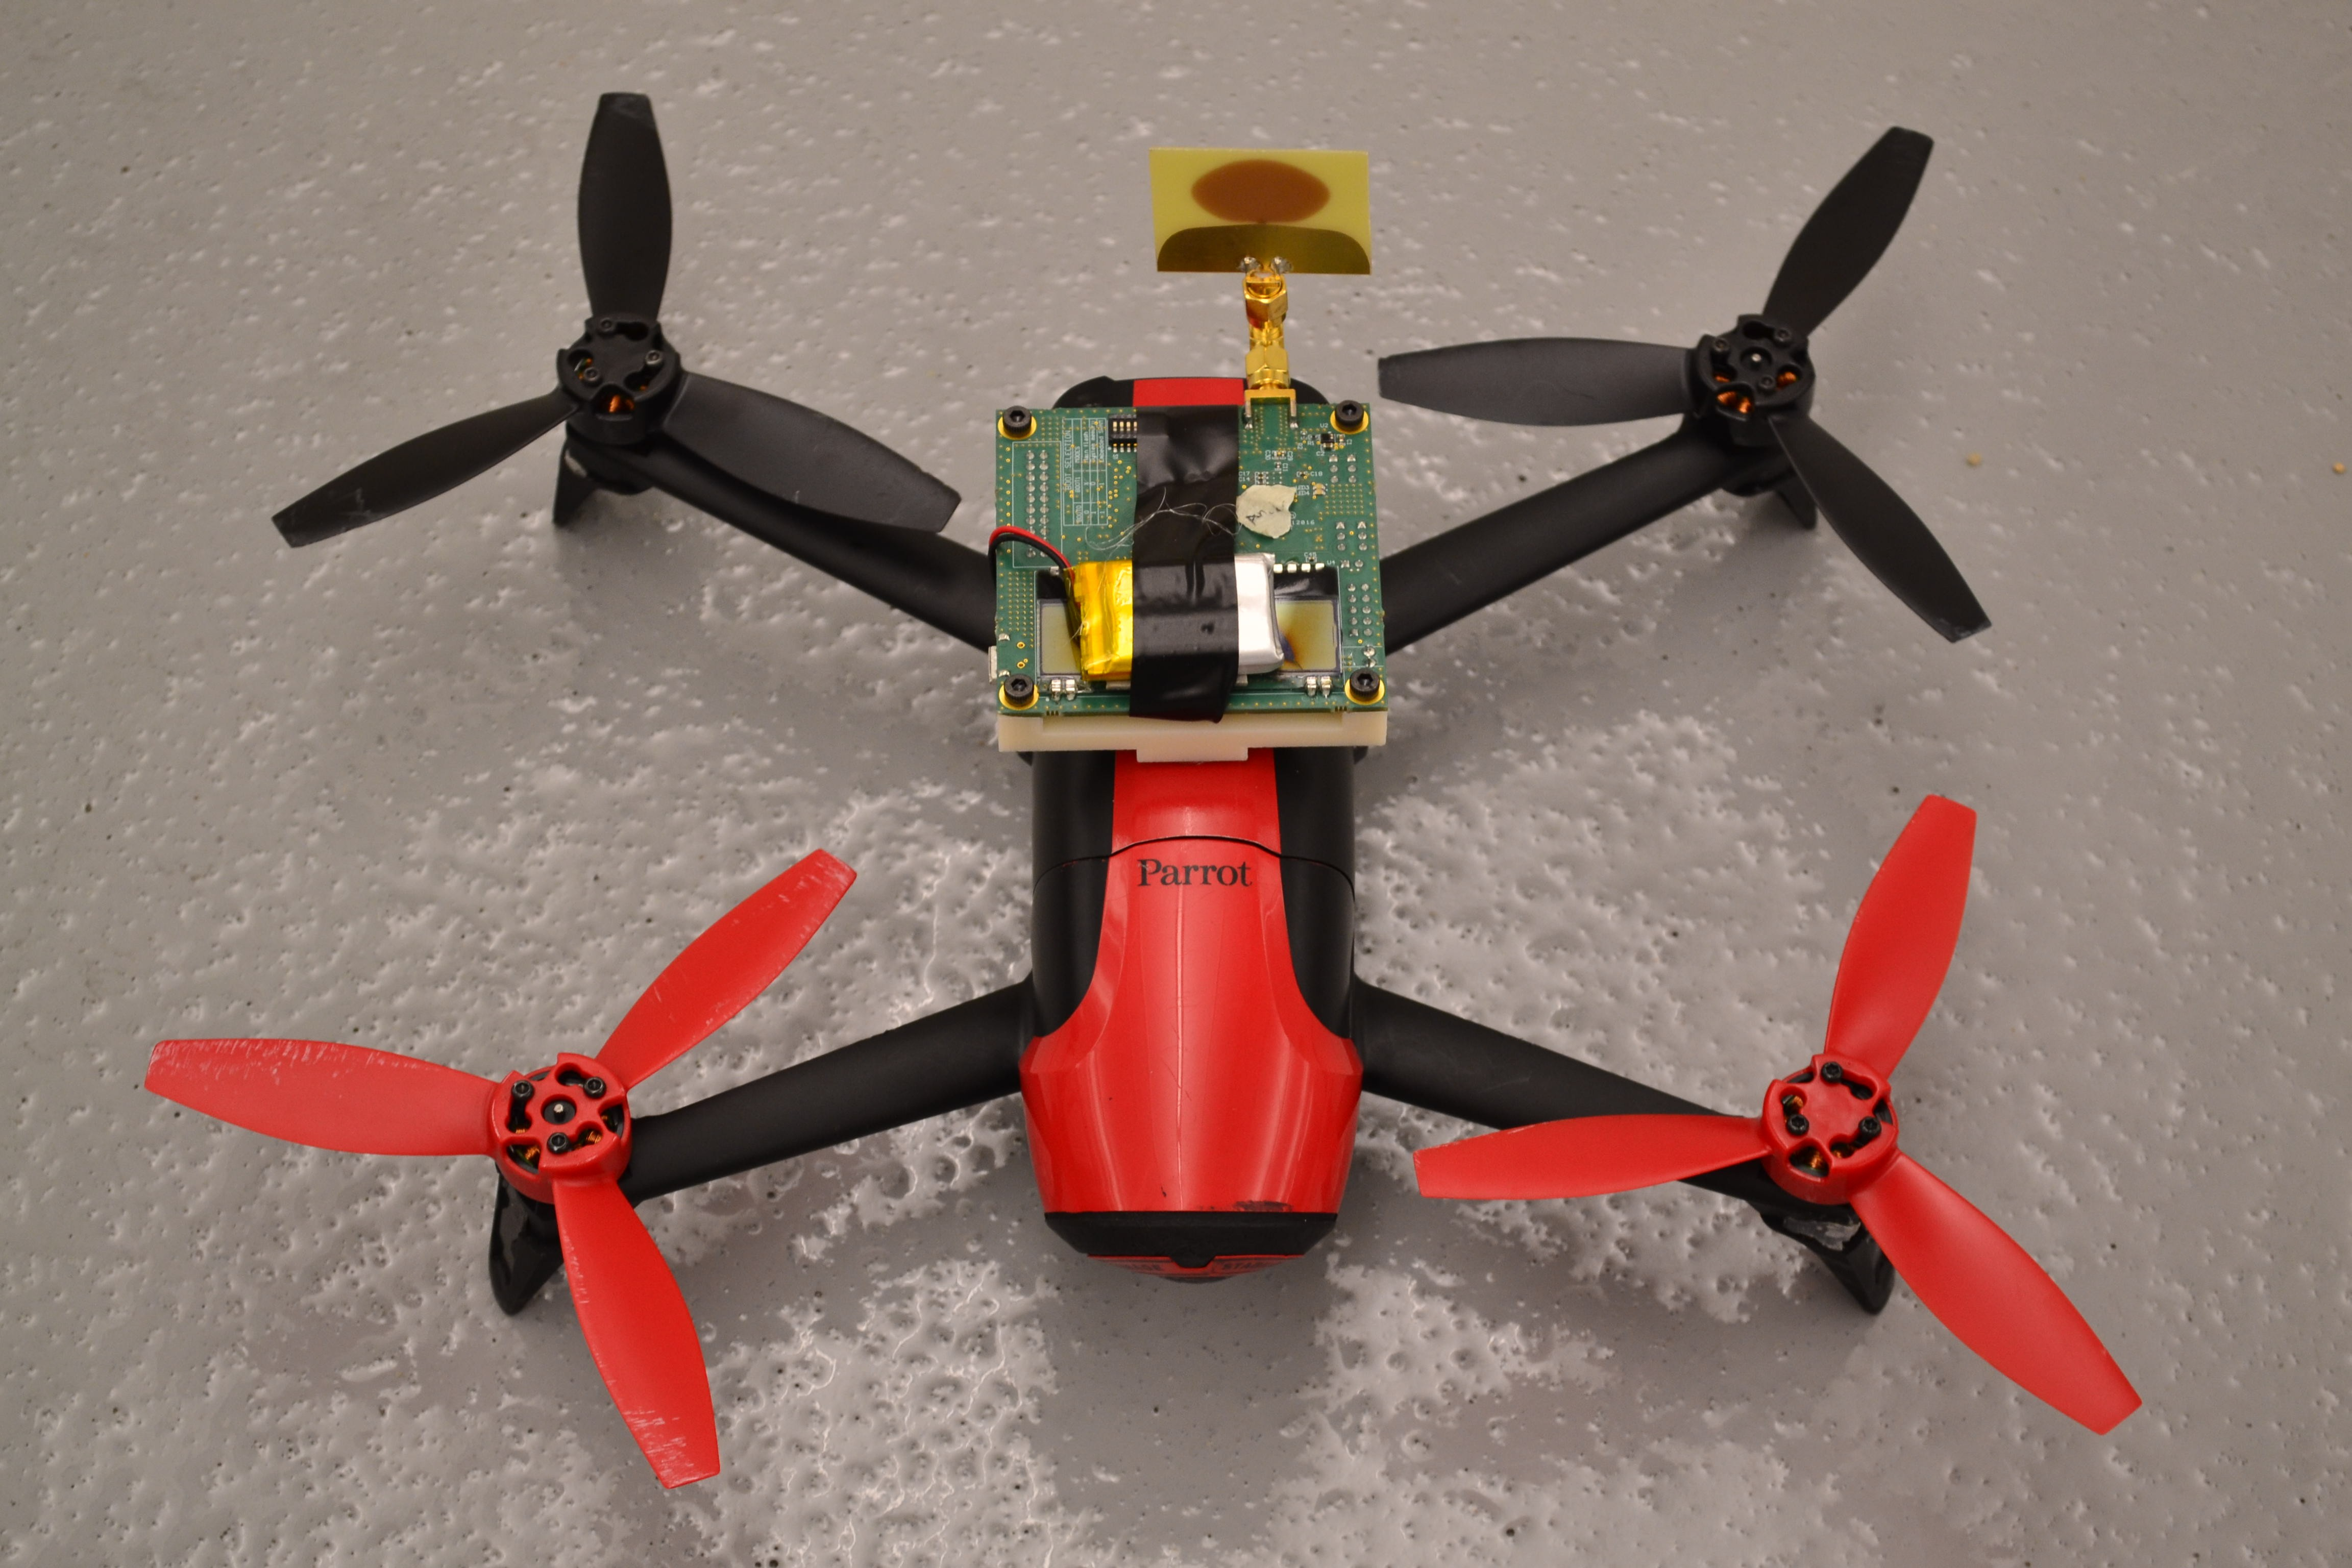
\includegraphics[width=0.9\linewidth]{bebop-actual}
    % 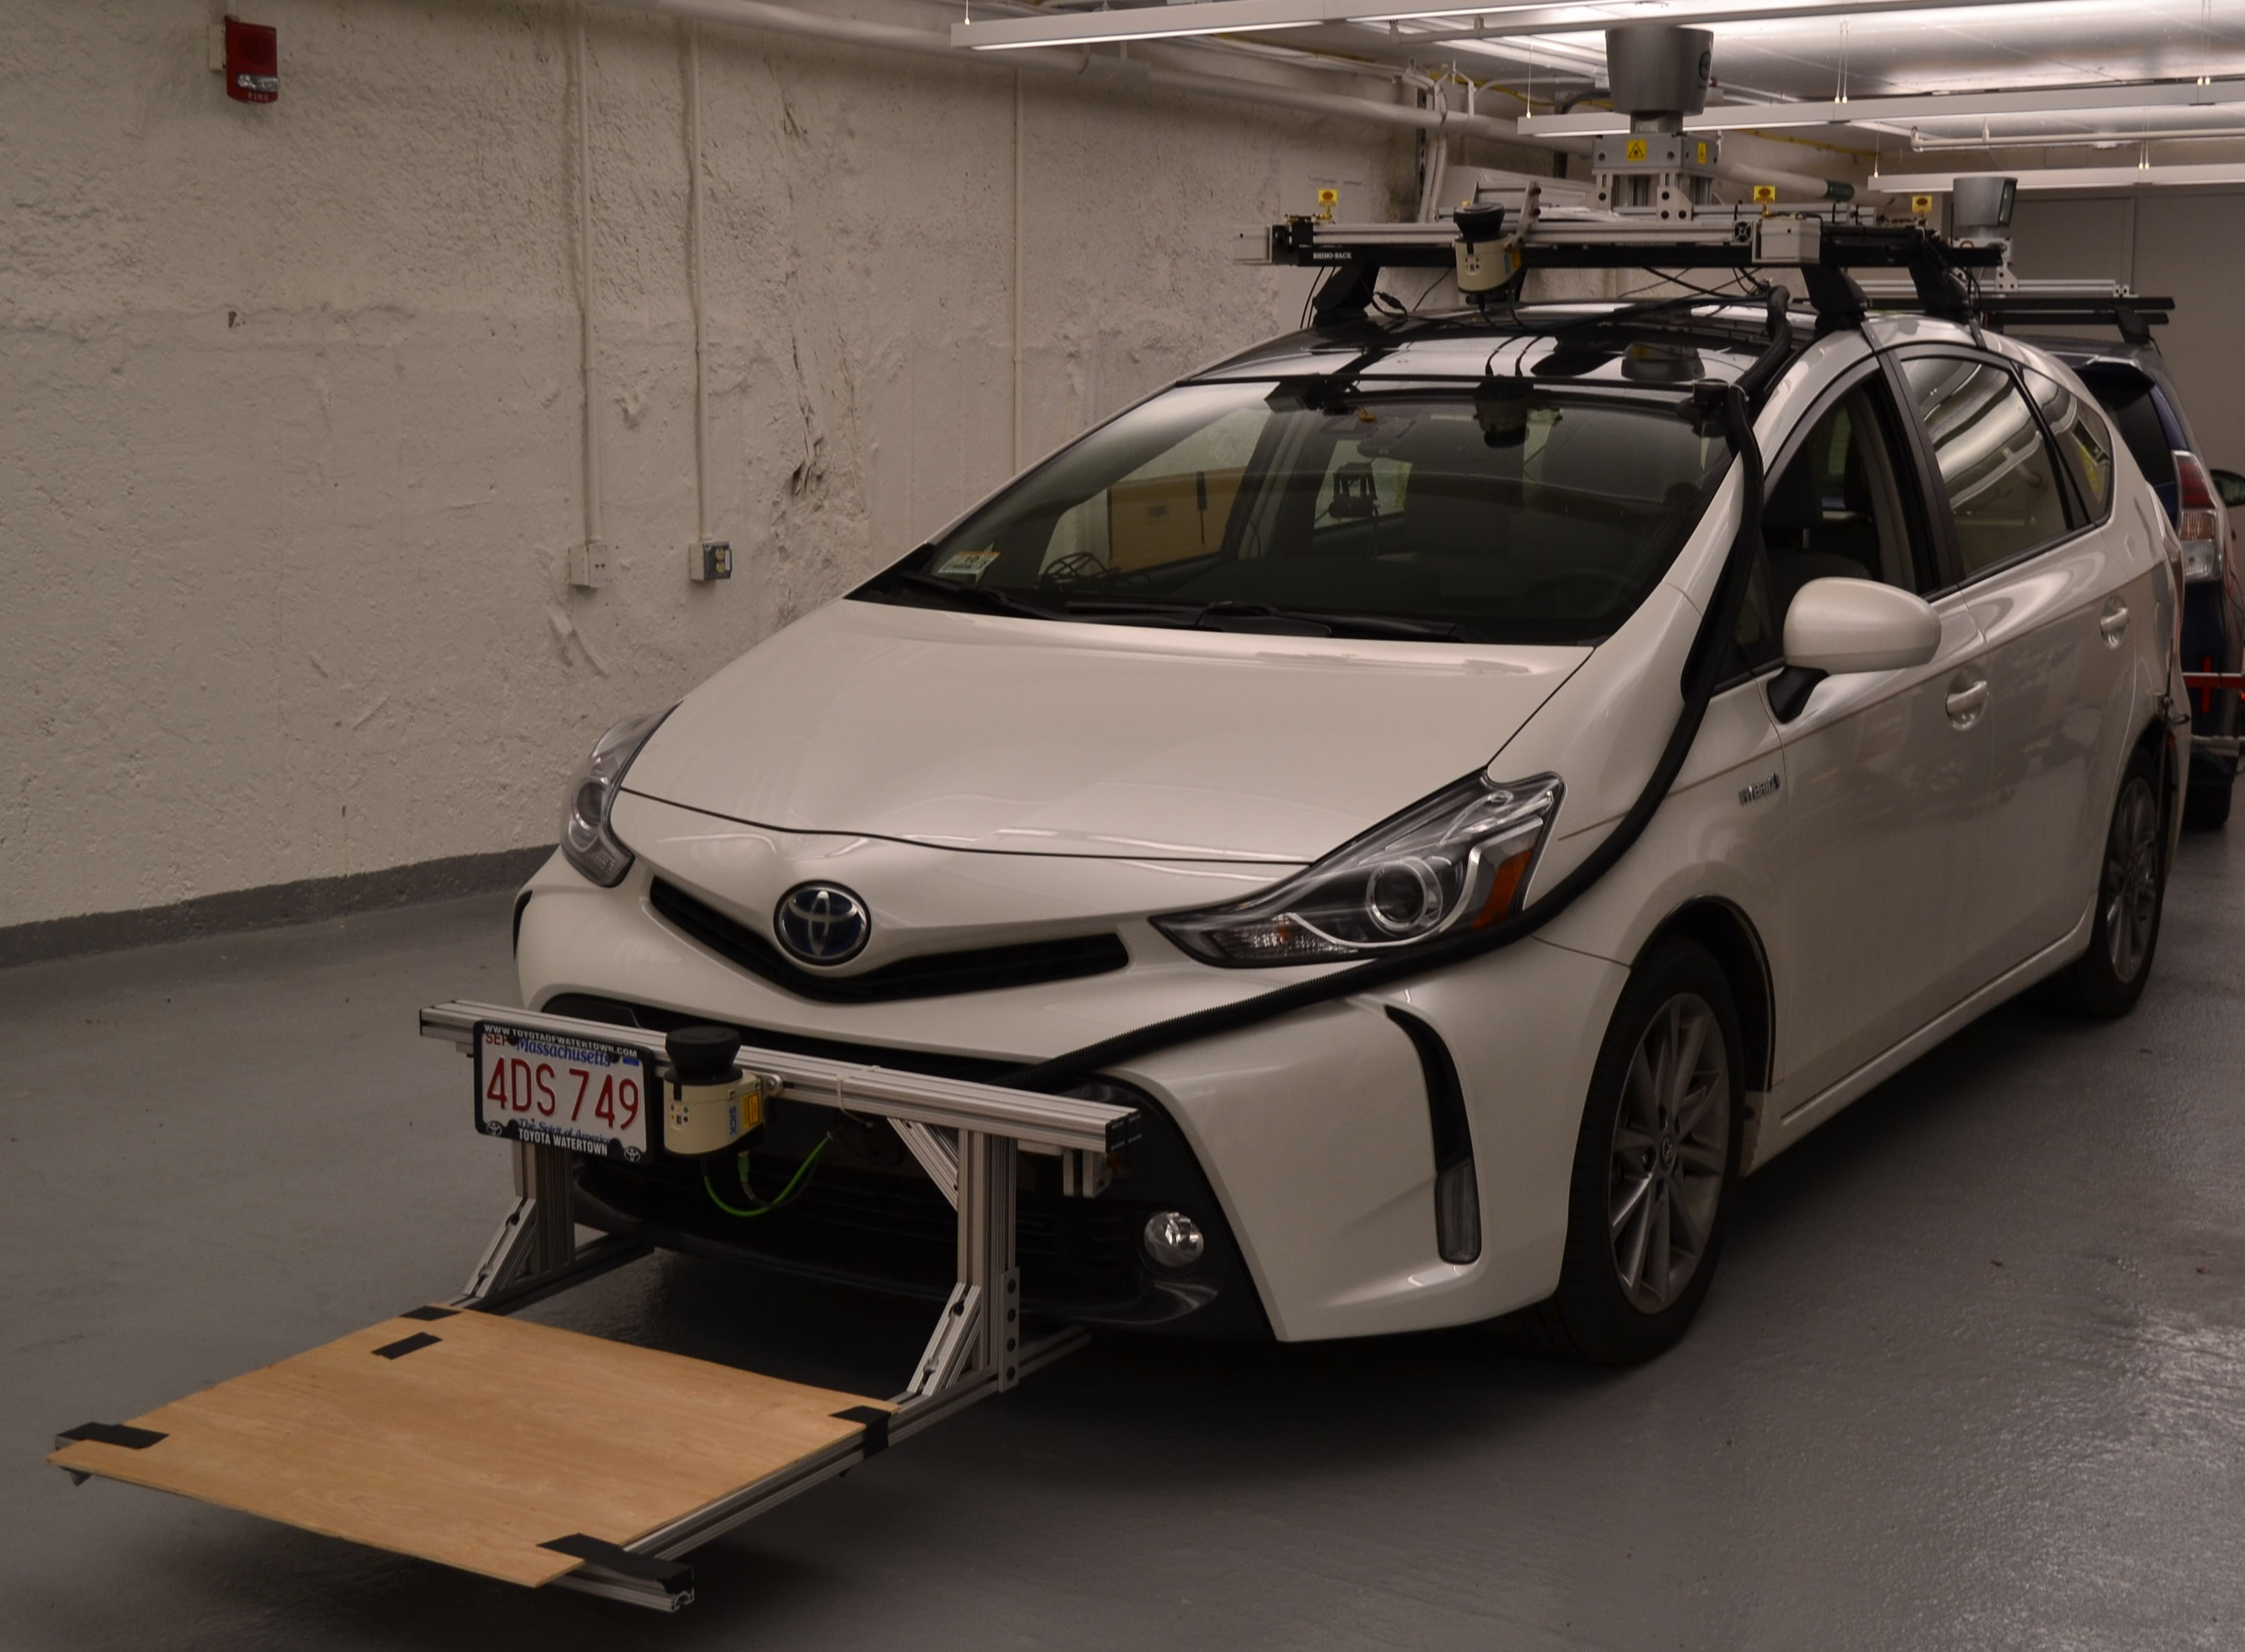
\includegraphics[height=3.8cm]{car}
    % 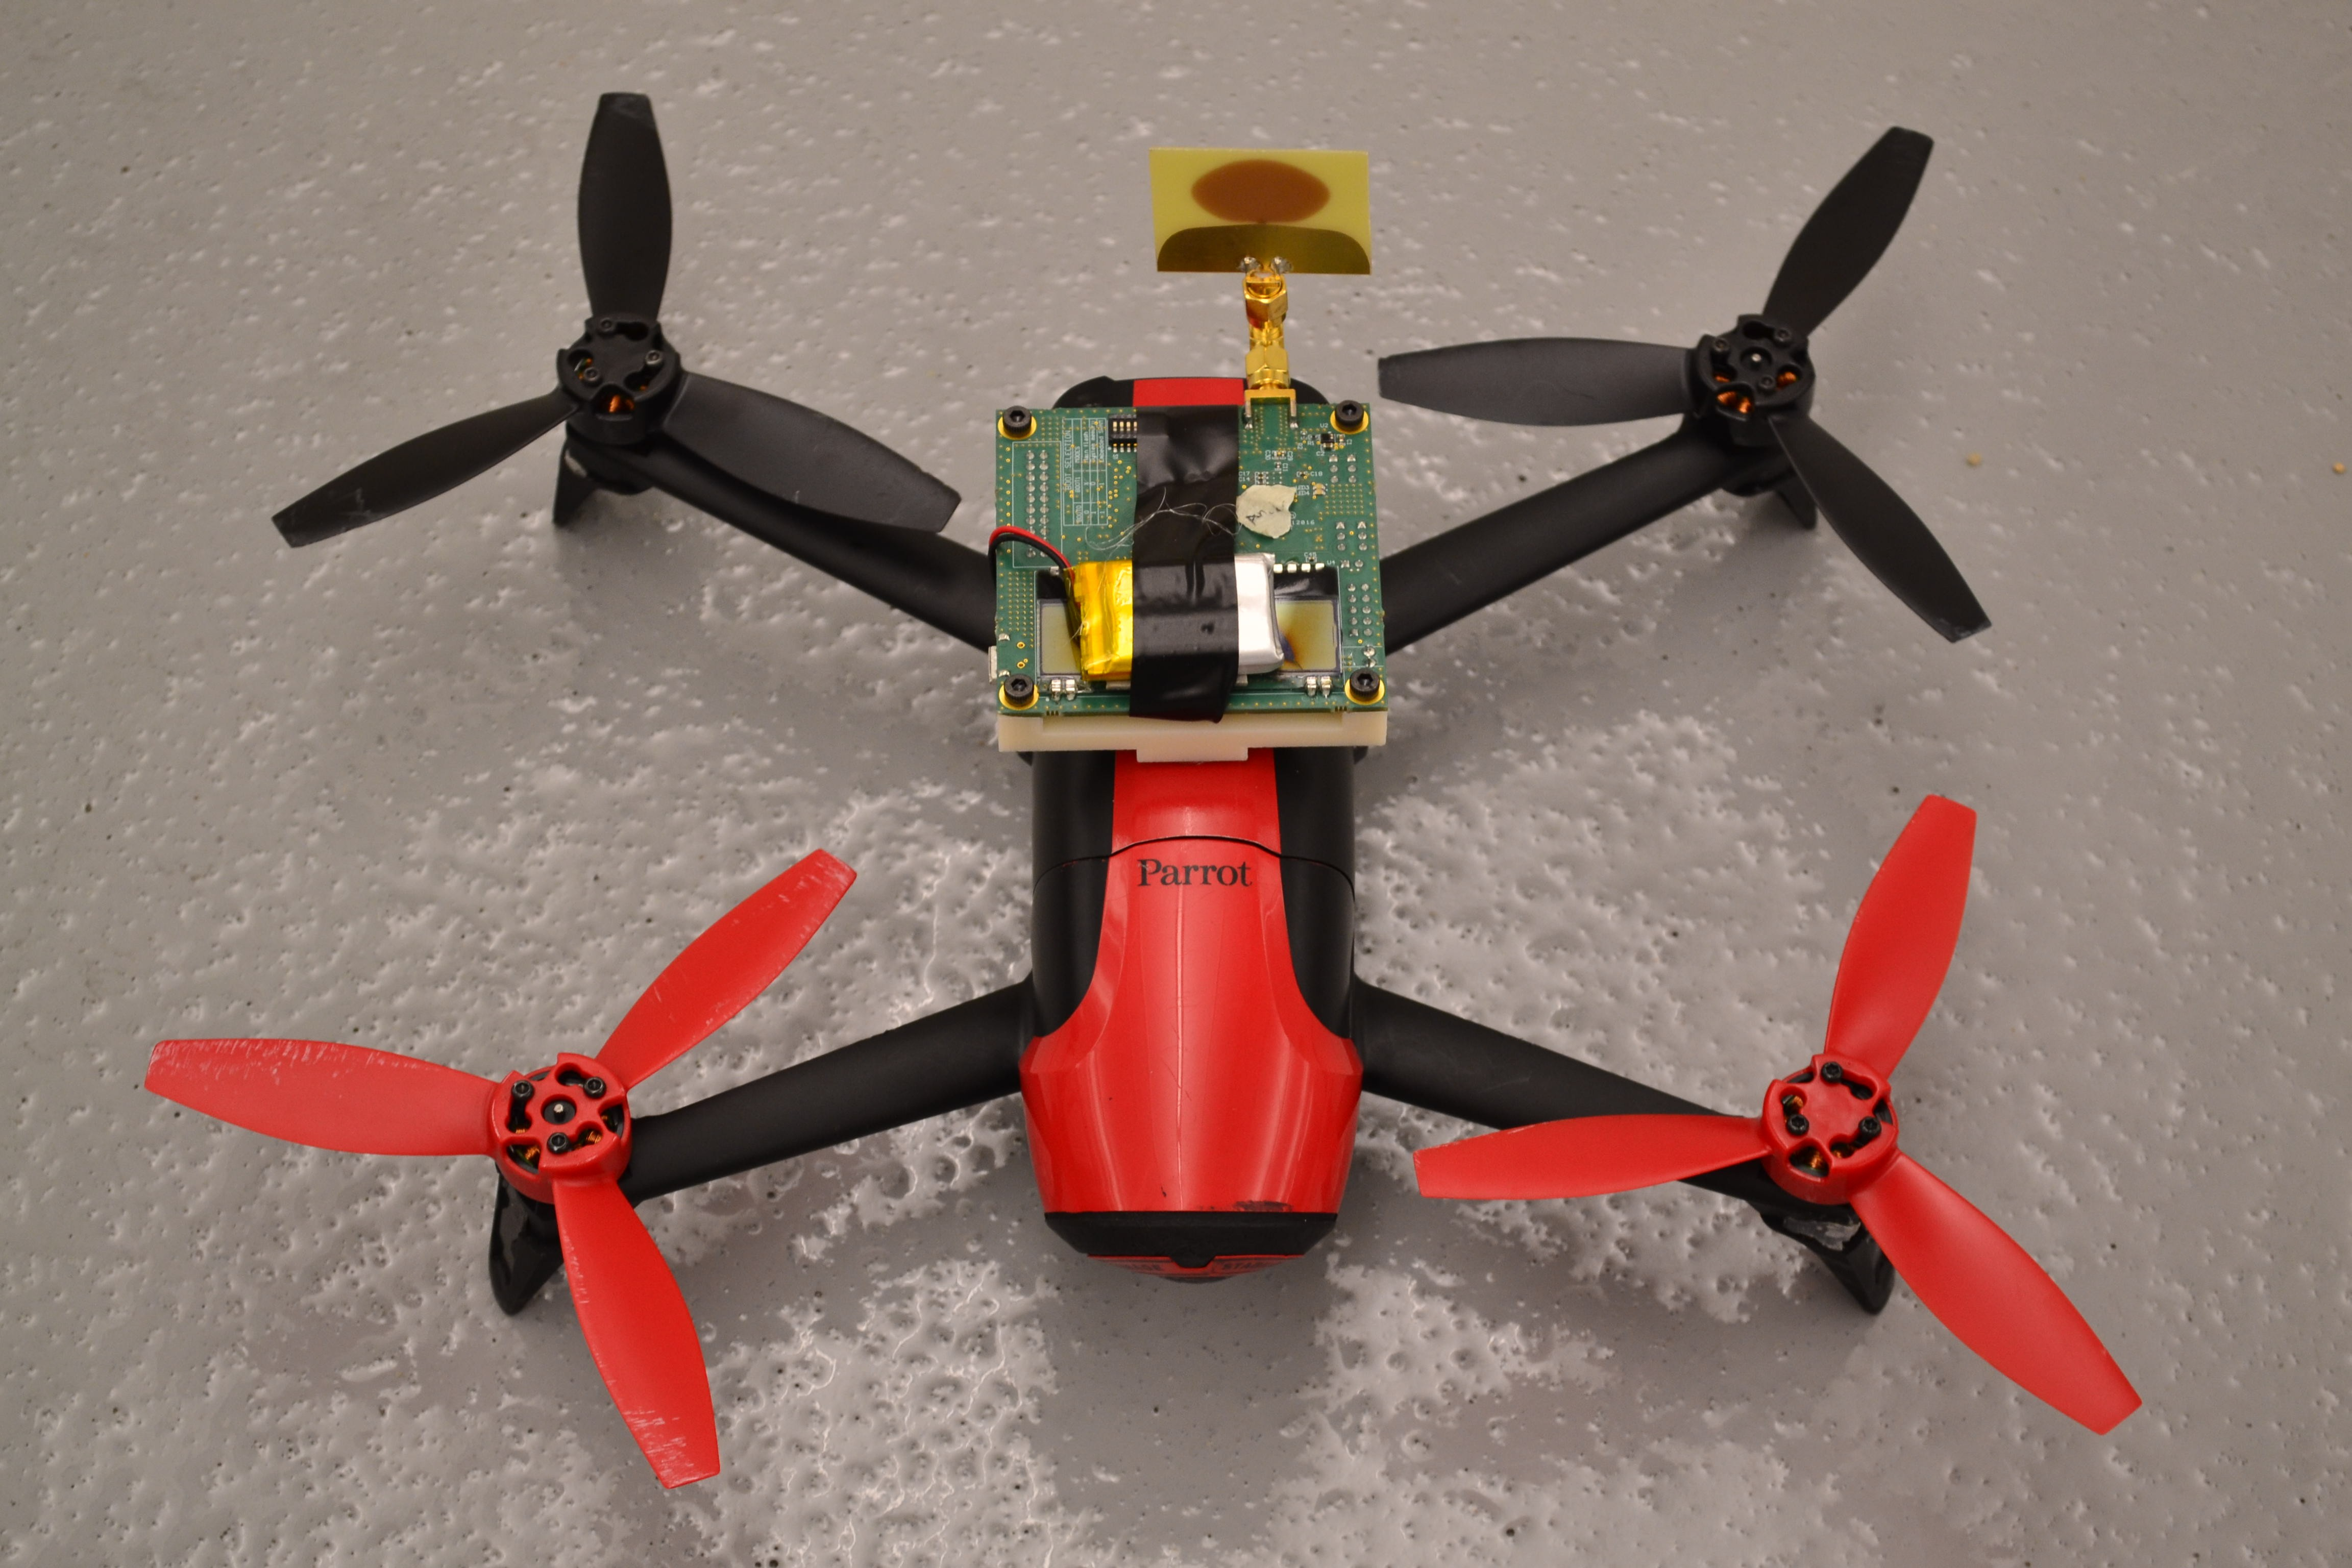
\includegraphics[height=3.8cm]{bebop-actual}

    \caption{}

    \label{fig:bebop-actual}

\end{figure}

Our experimental scenario involves a car preparing to leave a garage with a
significant blind spot. The car is unable to sense around the corner to
determine if there are pedestrians or other cars that may obstruct its path.
Our quadrotor takes off from the car's front bumper platform and autonomously
flies out of the garage and looks around the corner. The car is then able to
leave the garage when there are no more pedestrians detected by the quadrotor.
Once the car is ready to return, it backs up into the garage. The quadrotor
then follows the car into the garage and autonomously lands on the platform.

\subsection{Experiment With Actual Quadrotor}

\begin{figure}[h!]

    \centering

    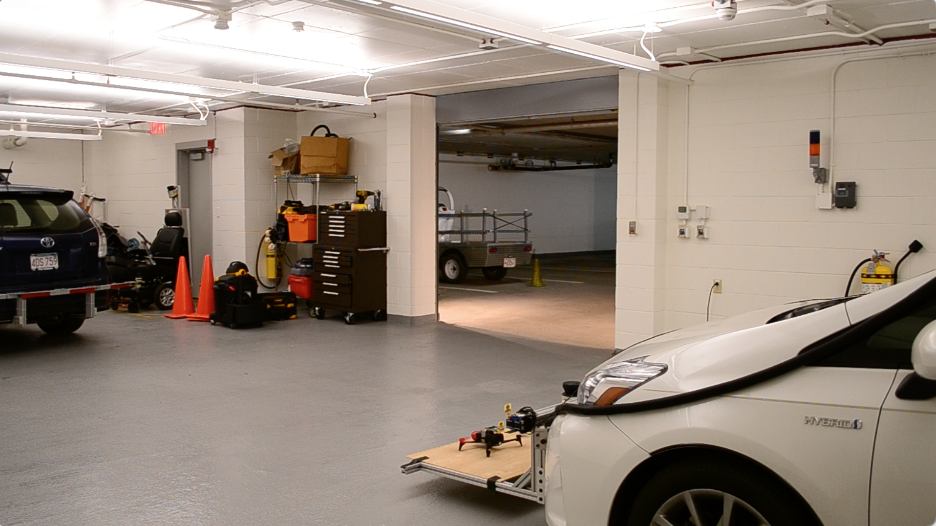
\includegraphics[width=0.3\linewidth]{00-third-person}
    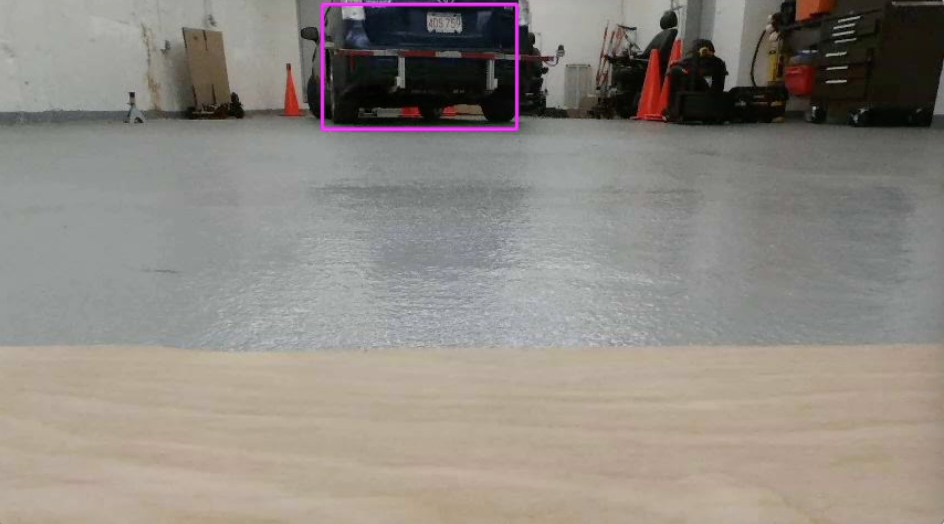
\includegraphics[width=0.3\linewidth]{00-quad-cam}
    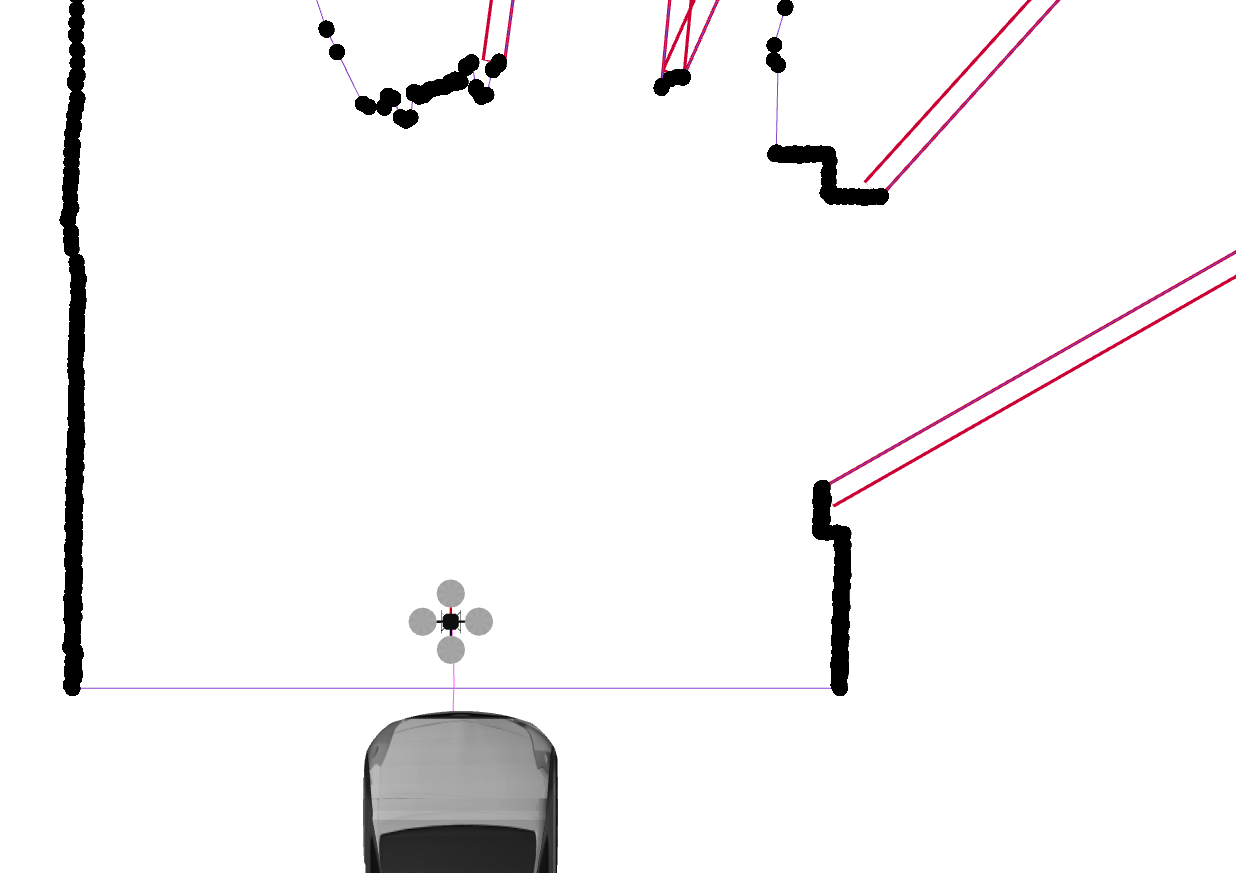
\includegraphics[width=0.3\linewidth]{00-planner-step} \\
    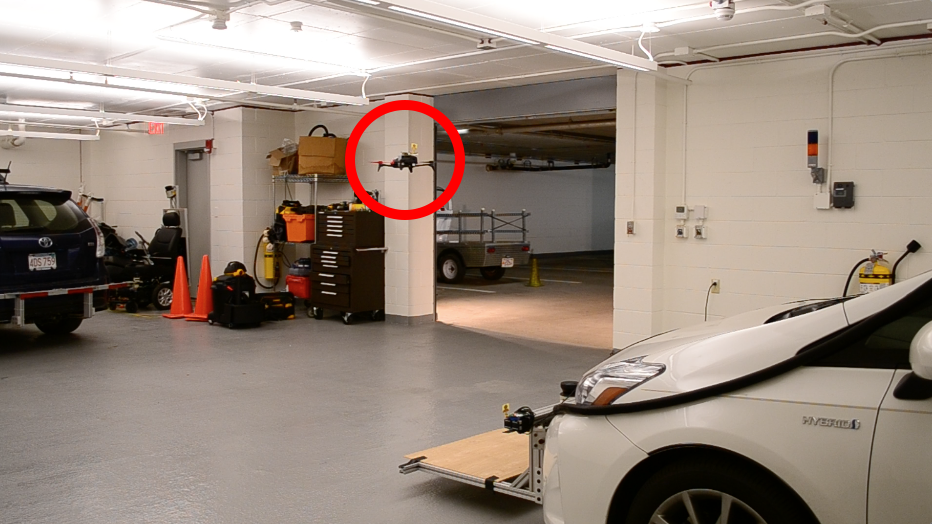
\includegraphics[width=0.3\linewidth]{01-third-person}
    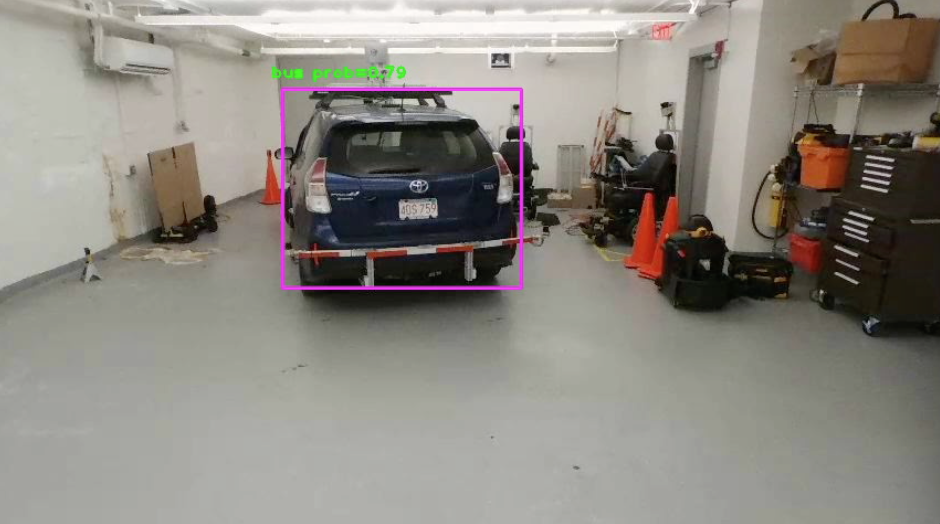
\includegraphics[width=0.3\linewidth]{01-quad-cam}
    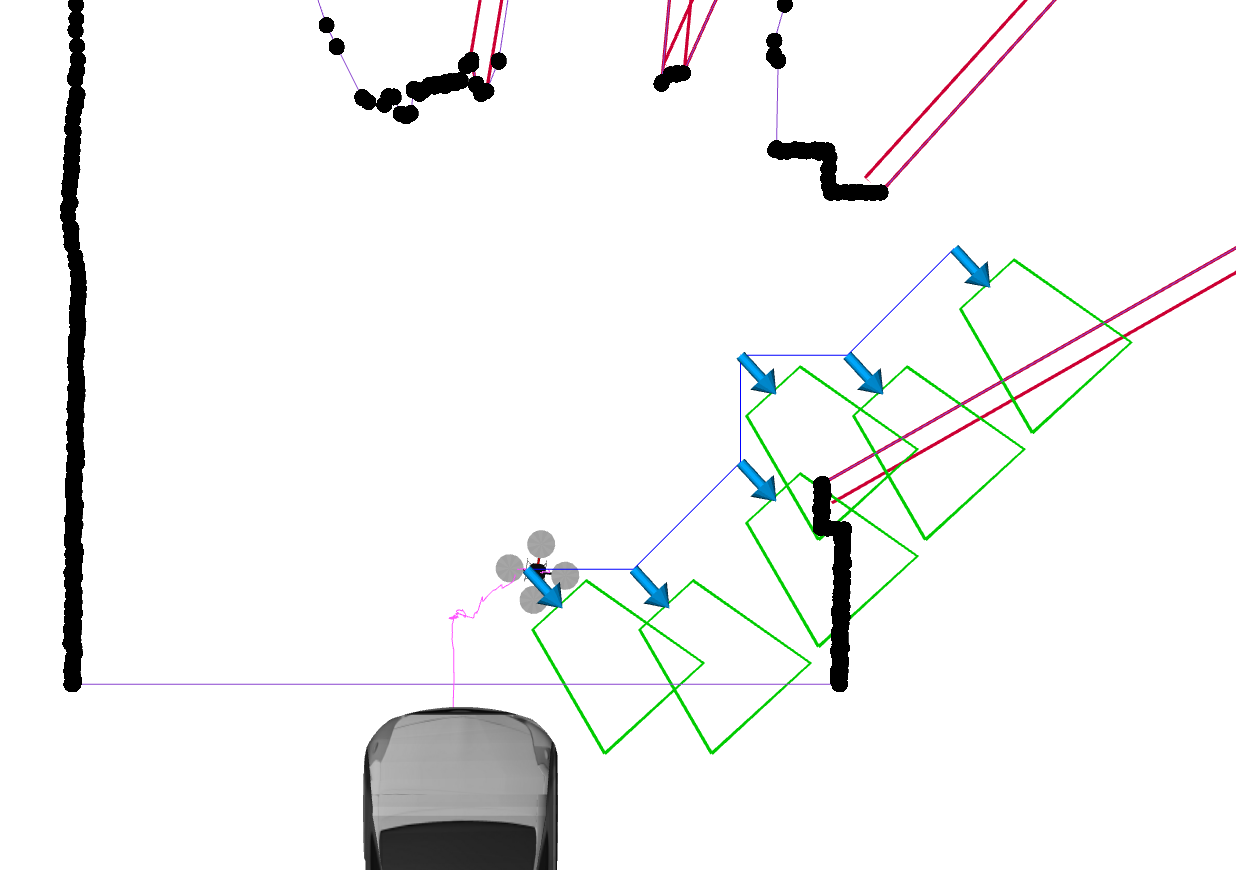
\includegraphics[width=0.3\linewidth]{01-planner-step} \\
    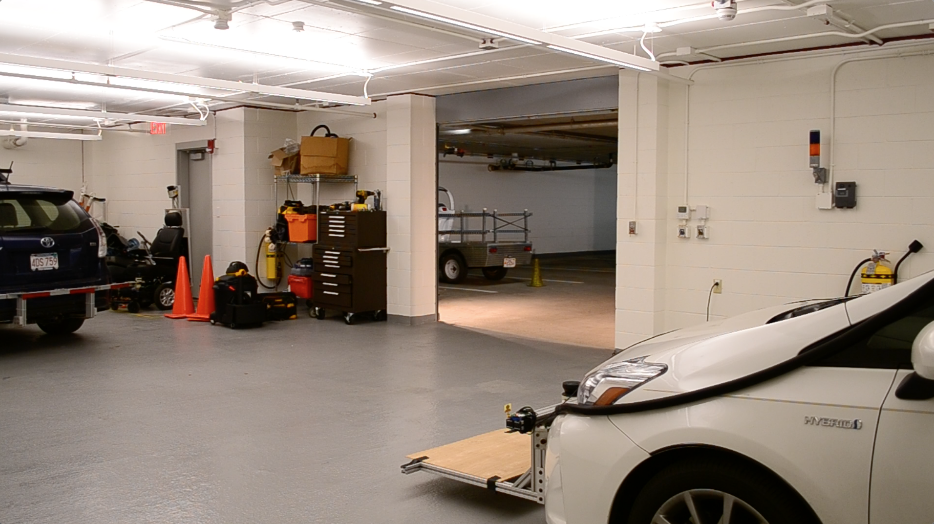
\includegraphics[width=0.3\linewidth]{02-third-person}
    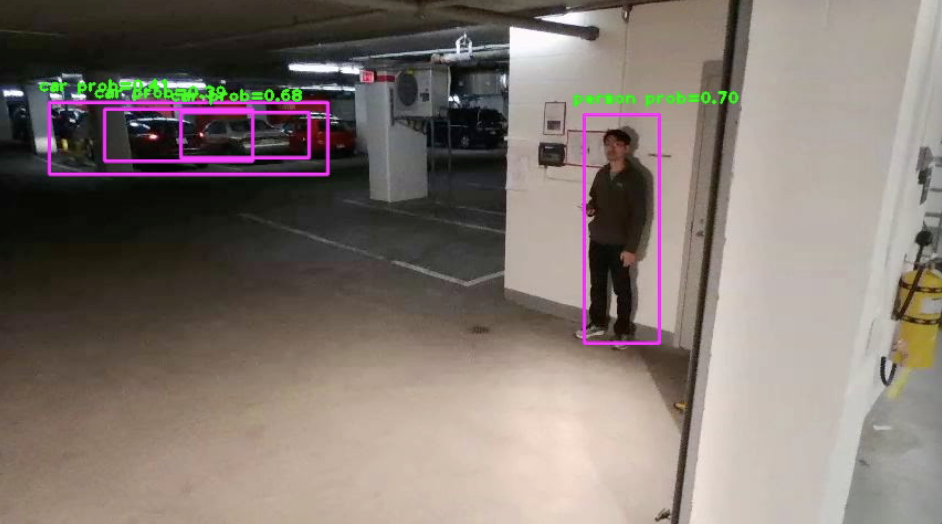
\includegraphics[width=0.3\linewidth]{02-quad-cam}
    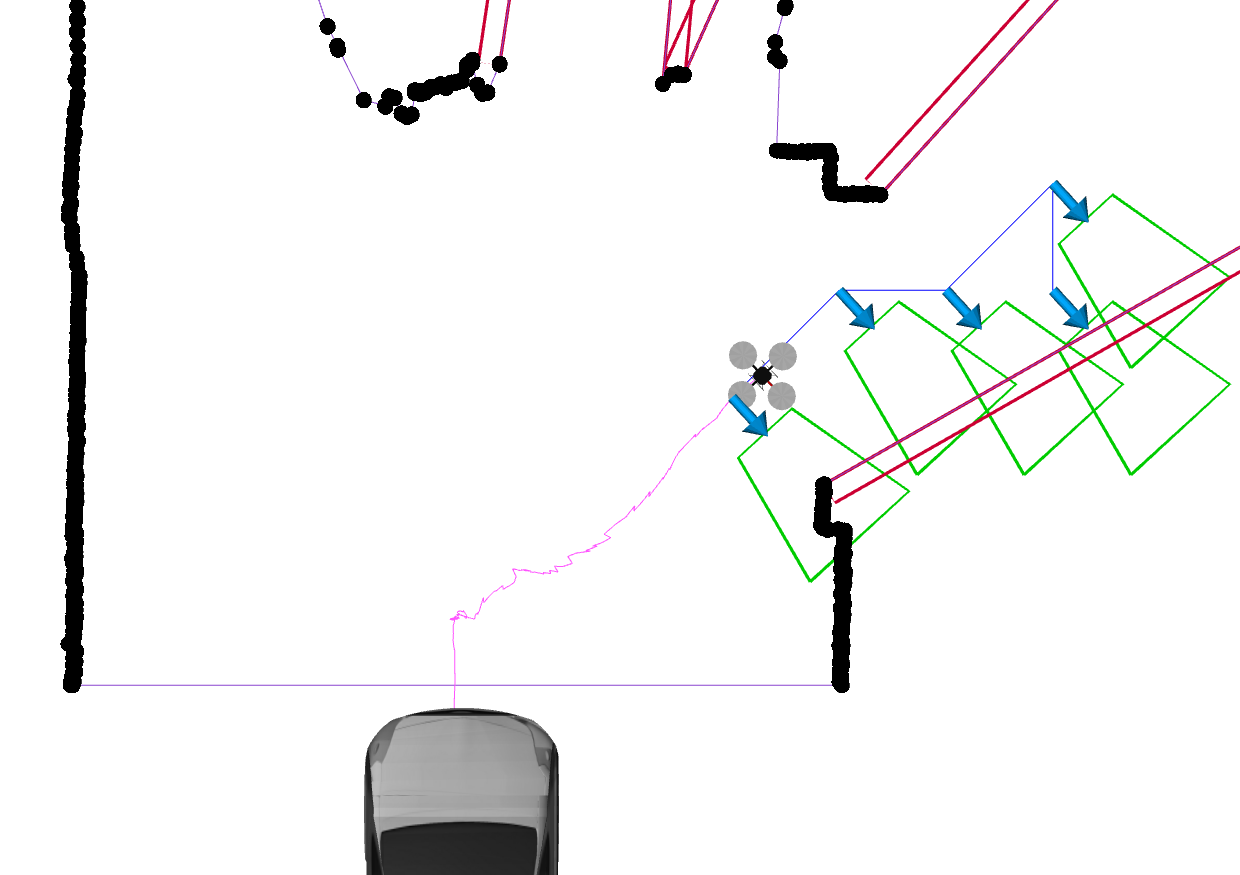
\includegraphics[width=0.3\linewidth]{02-planner-step}

\end{figure}
